\documentclass{beamer}
% Encodings (to render letters with diacritics and special characters)
\usepackage[utf8]{inputenc}
% Language
\usepackage[portuguese]{babel}

\usetheme{Madrid}
\usecolortheme{default}

\pdfstringdefDisableCommands{
  \def\\{}
  \def\texttt#1{<#1>}
}

\newcommand{\email}[1]{
{\footnotesize \texttt{\href{mailto:#1}{#1}} }
}

\usepackage{caption}
\DeclareCaptionFont{black}{\color{black}}
\DeclareCaptionFormat{listing}{{\tiny \textbf{#1}#2#3}}
\captionsetup[lstlisting]{format=listing,labelfont=black,textfont=black}

\usepackage{listings}
\lstset{
    frame=tb, % draw frame at top and bottom of the code
    basewidth  = {0.5em,0.5em},
    numbers=left, % display line numbers on the left
    showstringspaces=false, % don't mark spaces in strings  
    commentstyle=\color{green}, % comment color
    keywordstyle=\color{blue}, % keyword color
    stringstyle=\color{red}, % string color
	aboveskip=-0.2em,
    belowskip=-0.2em,
    basicstyle=\tiny
}
\lstset{literate=
  {á}{{\'a}}1 {é}{{\'e}}1 {í}{{\'i}}1 {ó}{{\'o}}1 {ú}{{\'u}}1
  {Á}{{\'A}}1 {É}{{\'E}}1 {Í}{{\'I}}1 {Ó}{{\'O}}1 {Ú}{{\'U}}1
  {à}{{\`a}}1 {è}{{\`e}}1 {ì}{{\`i}}1 {ò}{{\`o}}1 {ù}{{\`u}}1
  {À}{{\`A}}1 {È}{{\'E}}1 {Ì}{{\`I}}1 {Ò}{{\`O}}1 {Ù}{{\`U}}1
  {ä}{{\"a}}1 {ë}{{\"e}}1 {ï}{{\"i}}1 {ö}{{\"o}}1 {ü}{{\"u}}1
  {Ä}{{\"A}}1 {Ë}{{\"E}}1 {Ï}{{\"I}}1 {Ö}{{\"O}}1 {Ü}{{\"U}}1
  {â}{{\^a}}1 {ê}{{\^e}}1 {î}{{\^i}}1 {ô}{{\^o}}1 {û}{{\^u}}1
  {Â}{{\^A}}1 {Ê}{{\^E}}1 {Î}{{\^I}}1 {Ô}{{\^O}}1 {Û}{{\^U}}1
  {Ã}{{\~A}}1 {ã}{{\~a}}1 {Õ}{{\~O}}1 {õ}{{\~o}}1
  {œ}{{\oe}}1 {Œ}{{\OE}}1 {æ}{{\ae}}1 {Æ}{{\AE}}1 {ß}{{\ss}}1
  {ű}{{\H{u}}}1 {Ű}{{\H{U}}}1 {ő}{{\H{o}}}1 {Ő}{{\H{O}}}1
  {ç}{{\c c}}1 {Ç}{{\c C}}1 {ø}{{\o}}1 {å}{{\r a}}1 {Å}{{\r A}}1
  {€}{{\euro}}1 {£}{{\pounds}}1 {«}{{\guillemotleft}}1
  {»}{{\guillemotright}}1 {ñ}{{\~n}}1 {Ñ}{{\~N}}1 {¿}{{?`}}1
}

\usepackage{dirtree}

\usepackage[style=british]{csquotes}

\usepackage{tabularx}

\usepackage{graphicx}
	\graphicspath{{./images/}{../documentacao/}}
 
%Information to be included in the title page:
\AtBeginDocument{
\title[Tema 5 (Parte 1)]{Empresa de Transporte de Mercadorias (Parte 1)}
\subtitle{Transportes SML}
\author[T5G3]{
\begin{tabular}{r l}
	\email{up201806429@fe.up.pt} & Diogo Miguel Ferreira Rodrigues        \\
	\email{up201806554@fe.up.pt} & Telmo Alexandre Espirito Santo Baptista\\
	\email{up201306340@fe.up.pt} & Luís Paulo da Rocha Miranda
\end{tabular}
}
\institute[FEUP/AEDA]{Faculdade de Engenharia da Universidade do Porto \\ Algoritmos e Estruturas de Dados (AEDA) - Turma 5, grupo 3} 
\date[16/nov/2019]{16 de novembro de 2019}
}

\begin{document}
\frame{\titlepage}

\begin{frame}
\frametitle{Problema: Empresa de Transporte de Mercadorias}
\begin{quote}
Modelar um problema recorrendo ao paradigma da orientação por objetos e usar a linguagem C++ para implementar a solução correspondente.
\end{quote}
\begin{quote}
A empresa Transportes SML é especialista no transporte de mercadorias. A empresa possui um número fixo de camiões de diferentes tipos, específicos para o transporte de determinada mercadoria [...]
\end{quote}
\begin{quote}
Os clientes podem requisitar serviços de transporte de mercadorias, o que pode obrigar ao uso de múltiplos camiões por parte da empresa.
\end{quote}
\begin{quote}
Interessa conhecer os valores mensais que a empresa retira dos seus serviços de transporte, para cada um dos tipos de camião e no geral. Deve ser possível monitorar os clientes da empresa e serviços efetuados.
\end{quote}
\end{frame}

\begin{frame}
\frametitle{Solução}
Os utilizadores da aplicação devem fazer login, e possuem permissões diferentes consoante o seu tipo:
\begin{itemize}
	\item Funcionário (\texttt{Employee})
	\begin{itemize}
		\item Gestor (\texttt{Manager})
		\item Condutor (\texttt{Driver})
	\end{itemize}
	\item Cliente (\texttt{Client})
\end{itemize}

Um só tipo de camiões (\texttt{Truck}), que pode carregar uma carga (\texttt{Cargo}) de um dos tipos, cujo preço de transporte varia:
\begin{itemize}
	\item Normal (\texttt{Normal})
	\item Animal (\texttt{Animal})
	\item Refrigerada (\texttt{Refrigerated})
	\item Perigoso (\texttt{Dangerous})
\end{itemize}

Quando um serviço (\texttt{Service}) é criado, são automaticamente atribuídos os camiões e condutores necessários. 
\end{frame}

\begin{frame}
\frametitle{Permissões}
\textbf{Todos os utilizadores}
\begin{itemize}
	\item Visualizar e alterar os seus dados pessoais
\end{itemize}

\textbf{Cliente}
\begin{itemize}
	\item Criar um novo serviço em seu nome
	\item Eliminar um serviço em seu nome
	\item Visualizar os seus serviços
\end{itemize}

\textbf{Condutor}
\begin{itemize}
	\item Visualizar os serviços que lhe foram atribuídos
	\item Visualizar a lista de camiões
\end{itemize}

\textbf{Gestor}
\begin{itemize}
	\item Criar e eliminar serviço em nome de qualquer cliente
	\item Criar, editar e eliminar clientes, condutores, gestores e camiões
	\item Visualizar todos os clientes, condutores, gestores, camiões e serviços
\end{itemize}
\end{frame}

\begin{frame}
\frametitle{Diagramas de herança}
\begin{center}
\centering
$\vcenter{\hbox{\includegraphics[scale=0.3]{{inherit_graph_2}}}}$ \hspace*{12px}
$\vcenter{\hbox{\includegraphics[scale=0.3]{{classCargo__inherit__graph}}}}$
\end{center}
\begin{center}
\centering
$\vcenter{\hbox{\includegraphics[scale=0.3]{{classPerson__inherit__graph}}}}$\hspace*{12px}
$\vcenter{\hbox{\includegraphics[scale=0.3]{{inherit_graph_13}}}}$\hspace*{12px}
$\vcenter{\hbox{\includegraphics[scale=0.3]{{classutils_1_1string__regex__inherit__graph}}}}$
\end{center}
\end{frame}

\begin{frame}
\frametitle{Diagrama de classes \texttt{Cargo} e \texttt{Truck}}
\begin{center} \includegraphics[scale=0.36]{{Cargo_Truck_class_diagram}} \end{center}
\end{frame}

\begin{frame}
\frametitle{Diagrama de classes \texttt{Person}}
\begin{center} \includegraphics[scale=0.35]{{Person_class_diagram}} \end{center}
\end{frame}

\begin{frame}
\frametitle{Diagrama de classes \texttt{Service}}
\begin{center} \includegraphics[scale=0.37]{{Service_class_diagram}} \end{center}
\end{frame}

\begin{frame}
\frametitle{Diagrama de classes \texttt{utils::string\_regex}}
\begin{center} \includegraphics[scale=0.40]{{string_regex_class_diagram}} \end{center}
\end{frame}

\begin{frame}
\frametitle{Estrutura de ficheiros}
\begin{center}
\begin{minipage}{0.45\textwidth}
	\small
	\dirtree.
\begin{itemize}
	\item Resolve problema de ler linha completa de ficheiros
	\item Formato portável e independente da codificação do ficheiro
\end{itemize}
Convencionámos que, para as classes que implementámos, os operadores \texttt{<<}, \texttt{>>} seriam utilizados para I/O de ficheiros, em vez de I/O para o utilizador/linha de comandos
\end{minipage}
\end{center}
\end{frame}

\begin{frame}[fragile]
\begin{center}
\begin{tabular}{p{60mm} p{0mm} p{40mm}}
	\texttt{Person} & & \\	
	\lstinputlisting[aboveskip=-1em, belowskip=-1em, firstline=6, lastline=7]{../codigo/data/services/services.txt} & &
\begin{lstlisting}[aboveskip=-1em,belowskip=-1em]
Nome
Número de telemóvel
\end{lstlisting} \\
	\texttt{Client} & & \\
	\lstinputlisting[aboveskip=-1em, belowskip=-1em, firstline=30,lastline=37]{../codigo/data/clients/clients.txt} & &
\begin{lstlisting}[aboveskip=-1em,belowskip=-1em]
Nome
Número de telemóvel
Username
Password
Rua/porta
Código postal/Localidade
Região/País
NIF
\end{lstlisting} \\
	\texttt{Driver/Manager} & & \\
	\lstinputlisting[aboveskip=-1em, belowskip=-1em, firstline=3,lastline=11]{../codigo/data/managers/managers.txt} & &
\begin{lstlisting}[aboveskip=-1em,belowskip=-1em]
Nome
Número de telemóvel
Username
Password
Rua/porta
Código postal/Localidade
Região/País
NIF
Salário base
\end{lstlisting}
\end{tabular}
\end{center}
\end{frame}

\begin{frame}[fragile]
\begin{center}
\begin{tabular}{p{60mm} p{0mm} p{40mm}}
	\texttt{Services} & & \\	
	\lstinputlisting[firstline=1,lastline=25]{../codigo/data/services/services.txt} & &
\begin{lstlisting}
ID do próx. serviço a adicionar
Número de serviços

ID do serviço
Username do cliente
  Nome do contacto 1
  Núm. telemóvel do contacto 1
  Nome do contacto 2
  Núm. telemóvel do contacto 2
Tempo de início
Tempo de fim
Morada de início: rua/porta
  Código postal/Localidade
  Região/País
Morada de fim: rua/porta
  Código postal/Localidade
  Região/País
Distância
  Tipo de carga (0 = Normal)
  Peso em quilogramas
  Descrição
  Número de camiões/condutores
    Camião / Condutor
  Custos para empresa
  Receita com serviço
\end{lstlisting}
\end{tabular}
\end{center}
\end{frame}
 
\begin{frame}
\frametitle{Exceções tratadas}
\texttt{App::InvalidCredentials}: introduzidas credenciais erradas\\
\texttt{App::RepeatedId}: detetado um ID repetido quando o ID é único\\
\texttt{Temperature::InvalidTemperature}\\
\texttt{TemperatureRange::InvalidTemperatureRange}: gama de temperaturas inválida\\
\texttt{Time::InvalidTimeFormat}: formato errado\\
\texttt{Time::InvalidTime}\\
\texttt{utils::ufloat<T>::InvalidUFloat}\\
\texttt{utils::string\_regex::FailedRegex}: string introduzida não corresponde a regex\\
\texttt{std::invalid\_argument}\\
\texttt{std::system\_error} 
\end{frame}

\begin{frame}
\frametitle{Exemplo de exceção: \texttt{utils::string\_regex::FailedRegex}}
\begin{center} \begin{minipage}{0.95\linewidth}
\lstinputlisting[language=C++, caption={utils.h, L239-254}, firstline=239, lastline=254]{../codigo/include/utils.h}
\lstinputlisting[language=C++, caption={utils.cpp, L129-134}, firstline=129, lastline=134]{../codigo/src/utils.cpp}
\end{minipage} \end{center}
\end{frame}

\begin{frame}
\frametitle{Lista de funcionalidades}
\textbf{Tabelas}
\begin{itemize}
	\item Visualizar tabelas detalhadas das entidades
	\item Ordenar e pesquisar elementos da tabela por uma das várias propriedades
	\item Ordenações e pesquisas sucessivas
	\item Na tabela de serviços:
	\begin{itemize}
		\item Visualizar serviços entre dois dias
		\item Visualizar custos e despesas, para cada serviço e no total da tabela
	\end{itemize} 
\end{itemize}
\textbf{CRUD}
\begin{itemize}
	\item Criar, ler, editar e eliminar:
	\begin{itemize}
		\item Clientes
		\item Condutores
		\item Gestores
	\end{itemize}
	\item Criar, ler e eliminar serviços
\end{itemize}
\textbf{Login}
Sistema de login com nome de utilizador (\texttt{Username}) e palavra-passe (\texttt{Password}) para clientes, condutores e gestores.
\end{frame}

\begin{frame}
\frametitle{Destaque de funcionalidades: tabelas}
\begin{center} 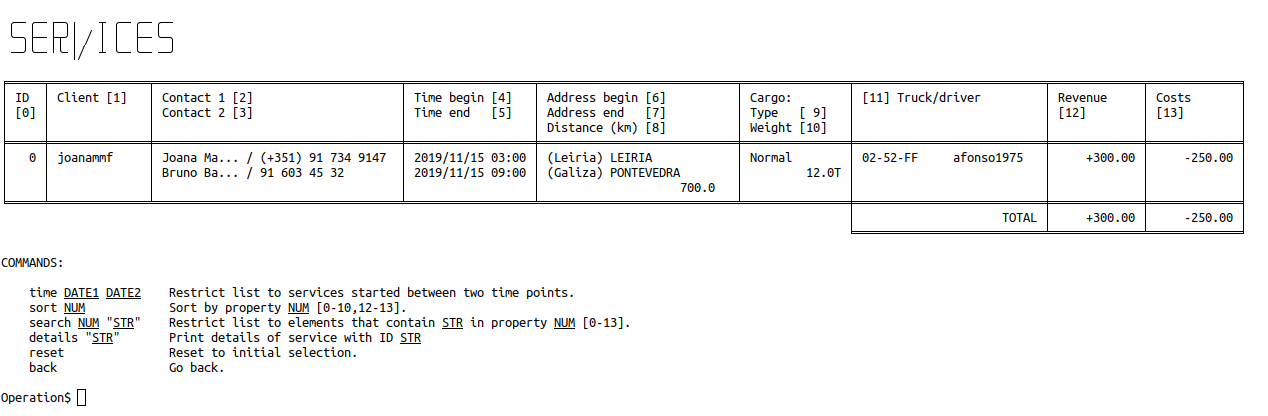
\includegraphics[scale=0.26]{feature1.png} \end{center}
\end{frame}

\begin{frame}
\begin{center} 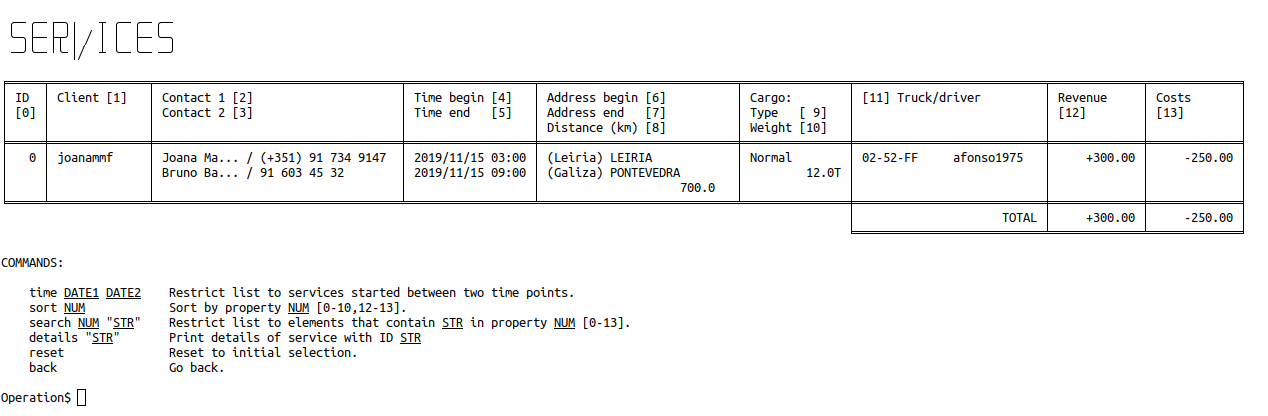
\includegraphics[scale=0.26]{feature1.png} \end{center}
\end{frame}

\begin{frame}
\begin{center} 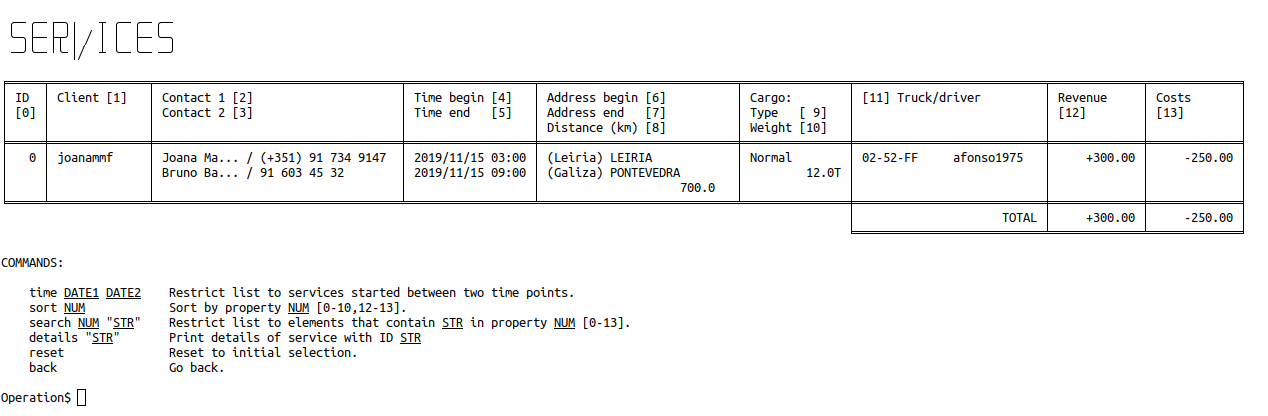
\includegraphics[scale=0.26]{feature1.png} \end{center}
\end{frame}

\begin{frame}
\frametitle{Destaque de funcionalidades: atribuição de serviços}
\begin{center}
\scalebox{.85}{
\lstinputlisting[language=C++, aboveskip=-1em, belowskip=-1em, caption={service.cpp, L81-111}, firstline=81, lastline=111]{../codigo/src/service.cpp}
}
\end{center}
\end{frame}

\begin{frame}
\frametitle{Dificuldades}
Trabalho de grupo
\begin{itemize}
	\item Componente colaborativa
	\item Componente individual
\end{itemize}
Existem muitas dependências entre classes e com a estrutura da aplicação.\\
Divisão de tarefas para componente individual mais difícil.\\
\textbf{Tempo}
\begin{itemize}
	\item Como gerir o tempo na aplicação?
	\item Pagar salários, notificar condutores dos seus futuros serviços
	\item Marcar serviços como concluídos, não concluídos, atrasados...
\end{itemize}
\end{frame}

\begin{frame}
\begin{minipage}[t]{0.33\linewidth}
	\textbf{Diogo Rodrigues}
	{\footnotesize \begin{itemize}
		\item \texttt{utils}: quase tudo, incluindo \texttt{string\_regex}, \texttt{mergesort}, \texttt{find\_if}		
		\item \texttt{Person} e todas as classes derivadas
		\item \texttt{Truck}: reescreveu
		\item \texttt{Cargo}: reescreveu				
		\item I/O ficheiros
		\item \texttt{App}: tabelas, opções das tabelas e mostrar detalhes de entidades
		\item \texttt{Time}, \texttt{Address}, \texttt{Phonenumber}, \texttt{Temperature}, \texttt{VAT}
		\item \texttt{Service} e função de atribuição
		\item Apresentação
	\end{itemize} }
\end{minipage}%
\begin{minipage}[t]{0.33\linewidth}
	\textbf{Telmo Baptista}
	{\footnotesize \begin{itemize}
		\item \texttt{utils}: algumas funções
		\item \texttt{App}: input do utilizador; adição, edição e remoção de entidades
		\item \texttt{Cargo}: implementou
		\item \texttt{Person}: alguns métodos
		\item \texttt{Time}: algumas funções
		\item \texttt{Truck}: implementou
	\end{itemize} }
\end{minipage}%
\begin{minipage}[t]{0.33\linewidth}
	\textbf{Luís Miranda}
	{\footnotesize \begin{itemize}
		\item Organização da app
		\item Permissões
		\item Dados
		\item Testes
		\item Apresentação
	\end{itemize} }
\end{minipage}
\end{frame}
\end{document}


